\documentclass[\main.tex]{subfiles}

\chapter{Fundamentação Teórica}

\section{Série Temporal}
Uma série temporal é uma sequência de dados numéricos ordenados sequencialmente ao longo do
tempo\cite{wikipedia_times_series}. A ordem dos dados é extremamente fundamental, ao contrário de modelos de regressão
linear. Alguns exemplos destas séries são o registo das alturas das ondes do oceano,
contagens de manchas solares, rastreio de dados meteorológicos ou medição de velocidades.\par
Dependendo se o interesse é entender um conjunto de dados ou fazer previsões, os objetivos
adotados são diferentes. Compreender um \textit{\gls{dataset}} , chamado de análise de séries
temporais, pode ajudar a fazer melhores previsões, no entanto, não é obrigatório e pode
resultar num grande investimento técnico em tempo e experiência não diretamente alinhado com
os resultados esperados, que é prever o futuro.\par


\subsection{Análise}
A análise de uma série temporal envolve o desenvolvimento de modelos que melhor capturam ou
descrevem a mesma observada a fim de compreender as causas subjacentes\cite{wikipedia_times_series}. Este campo de estudo
procura o \say{porquê} por trás de um conjunto de dados da série. Isto, geralmente, envolve fazer
suposições sobre a forma dos dados e decompô-la em componentes de constituição.\par
A qualidade de um modelo descritivo é determinada pelo quão bem ele descreve todos os dados
disponíveis e pela interpretação que fornece para informar melhor o domínio do problema.\par
De modo a realizar esta análise, existem alguns métodos que permitem extrair estatísticas
significativas, visualizar parte dos dados e exportar gráficos explicativos (e.g., gráficos
de linha, histogramas, diagramas de caixa, mapas de calor, gráficos de dispersão, gráficos
de autocorrelação)\cite{data_visualization}. Na figura 2.1 pode ser analisada uma série temporal através do gráfico
de linha representado.\par

\begin{figure}[h!]
\centering
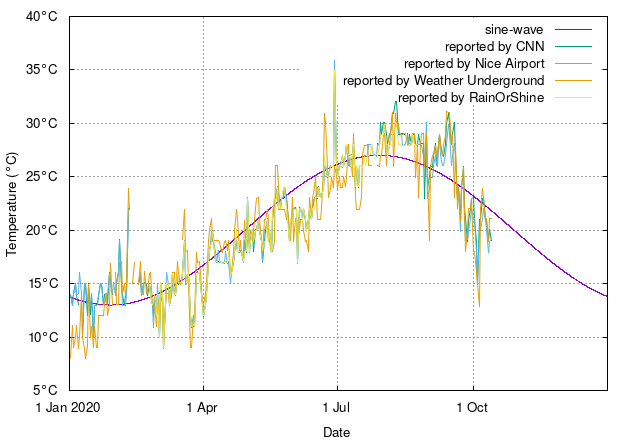
\includegraphics[width=0.8\linewidth]{../private_assets/timeseries_graph_example.png}
\caption{Temperaturas da cidade de Nice durante o ano atual}
\end{figure}\par


\subsection{Componentes}
Existem 4 componentes que uma série temporal pode ter\cite{timeseries_comp}:
\begin{itemize}
    \item Nível: valor base da série se fosse uma linha reta;
    \item Tendência (opcional): comportamento, normalmente linear, crescente ou decrescente
    ao longo do tempo;
    \item Sazonalidade (opcional): padrões repetitivos ou ciclos de comportamento ao longo
    do tempo;
    \item Ruído (opcional): variações nas observações que não podem ser explicadas pelo
    modelo.
\end{itemize}\par
Para concluir, todas as séries temporais têm nível e a maior parte também tem ruído.
No entanto, a tendência e a sazonalidade são ocasionais.\par


\subsection{Previsões}
Fazer previsões sobre o futuro é chamado de extrapolação no tratamento estatístico clássico
de dados de séries temporais. Campos mais modernos focam-se no tópico e referem-se a ele como
previsão destas séries. A previsão envolve o ajuste de modelos em dados históricos e o uso
destes dados para prever observações futuras. Posto isto, todos os dados de treino devem
permanecer guardados e ordenados temporalmente, para que não hajam problemas com as
previsões\cite{timeseries_forecast}.\par
Os modelos descritivos podem ser emprestados para o futuro, ou seja, para suavizar ou remover
o ruído. Um distinção importante na previsão é que o futuro está completamente indisponível e
deve ser estimado apenas a partir do que já aconteceu.\par
A habilidade de um modelo de previsão de série temporal é determinada pelo seu desempenho em
prever o futuro. Muitas vezes, isso ocorre às custas de ser capaz de explicar por que uma
previsão específica foi feita, os intervalos de confiança e ainda compreender as causas
subjacentes ao problema.\par
A previsão de séries temporais é uma área bastante importante de \textit{\acrfull{ml}} que
é frequentemente negligenciada. É muito importante, porque existem muitos problemas de
previsão que envolvem um componente de tempo. Esses problemas são esquecidos com
regularidade, pois é esse componente de tempo que os torna mais difíceis de resolver.\par
Para fazer previsões com séries temporais, é utilizado um modelo para prever valores
futuros com base em valores observados anteriormente. Na figura 2.2 está representado um
gráfico das previsões de vendas de um champô. A azul estão os dados de treino do modelo, a
verde estão os dados de teste e a vermelho as previsões realizadas pelo modelo. Este gráfico
foi retirado dos exercícios realizados pelo autor aquando do estudo do modelo
\textit{\acrshort{arima}}.\par

\begin{figure}[h!]
\centering
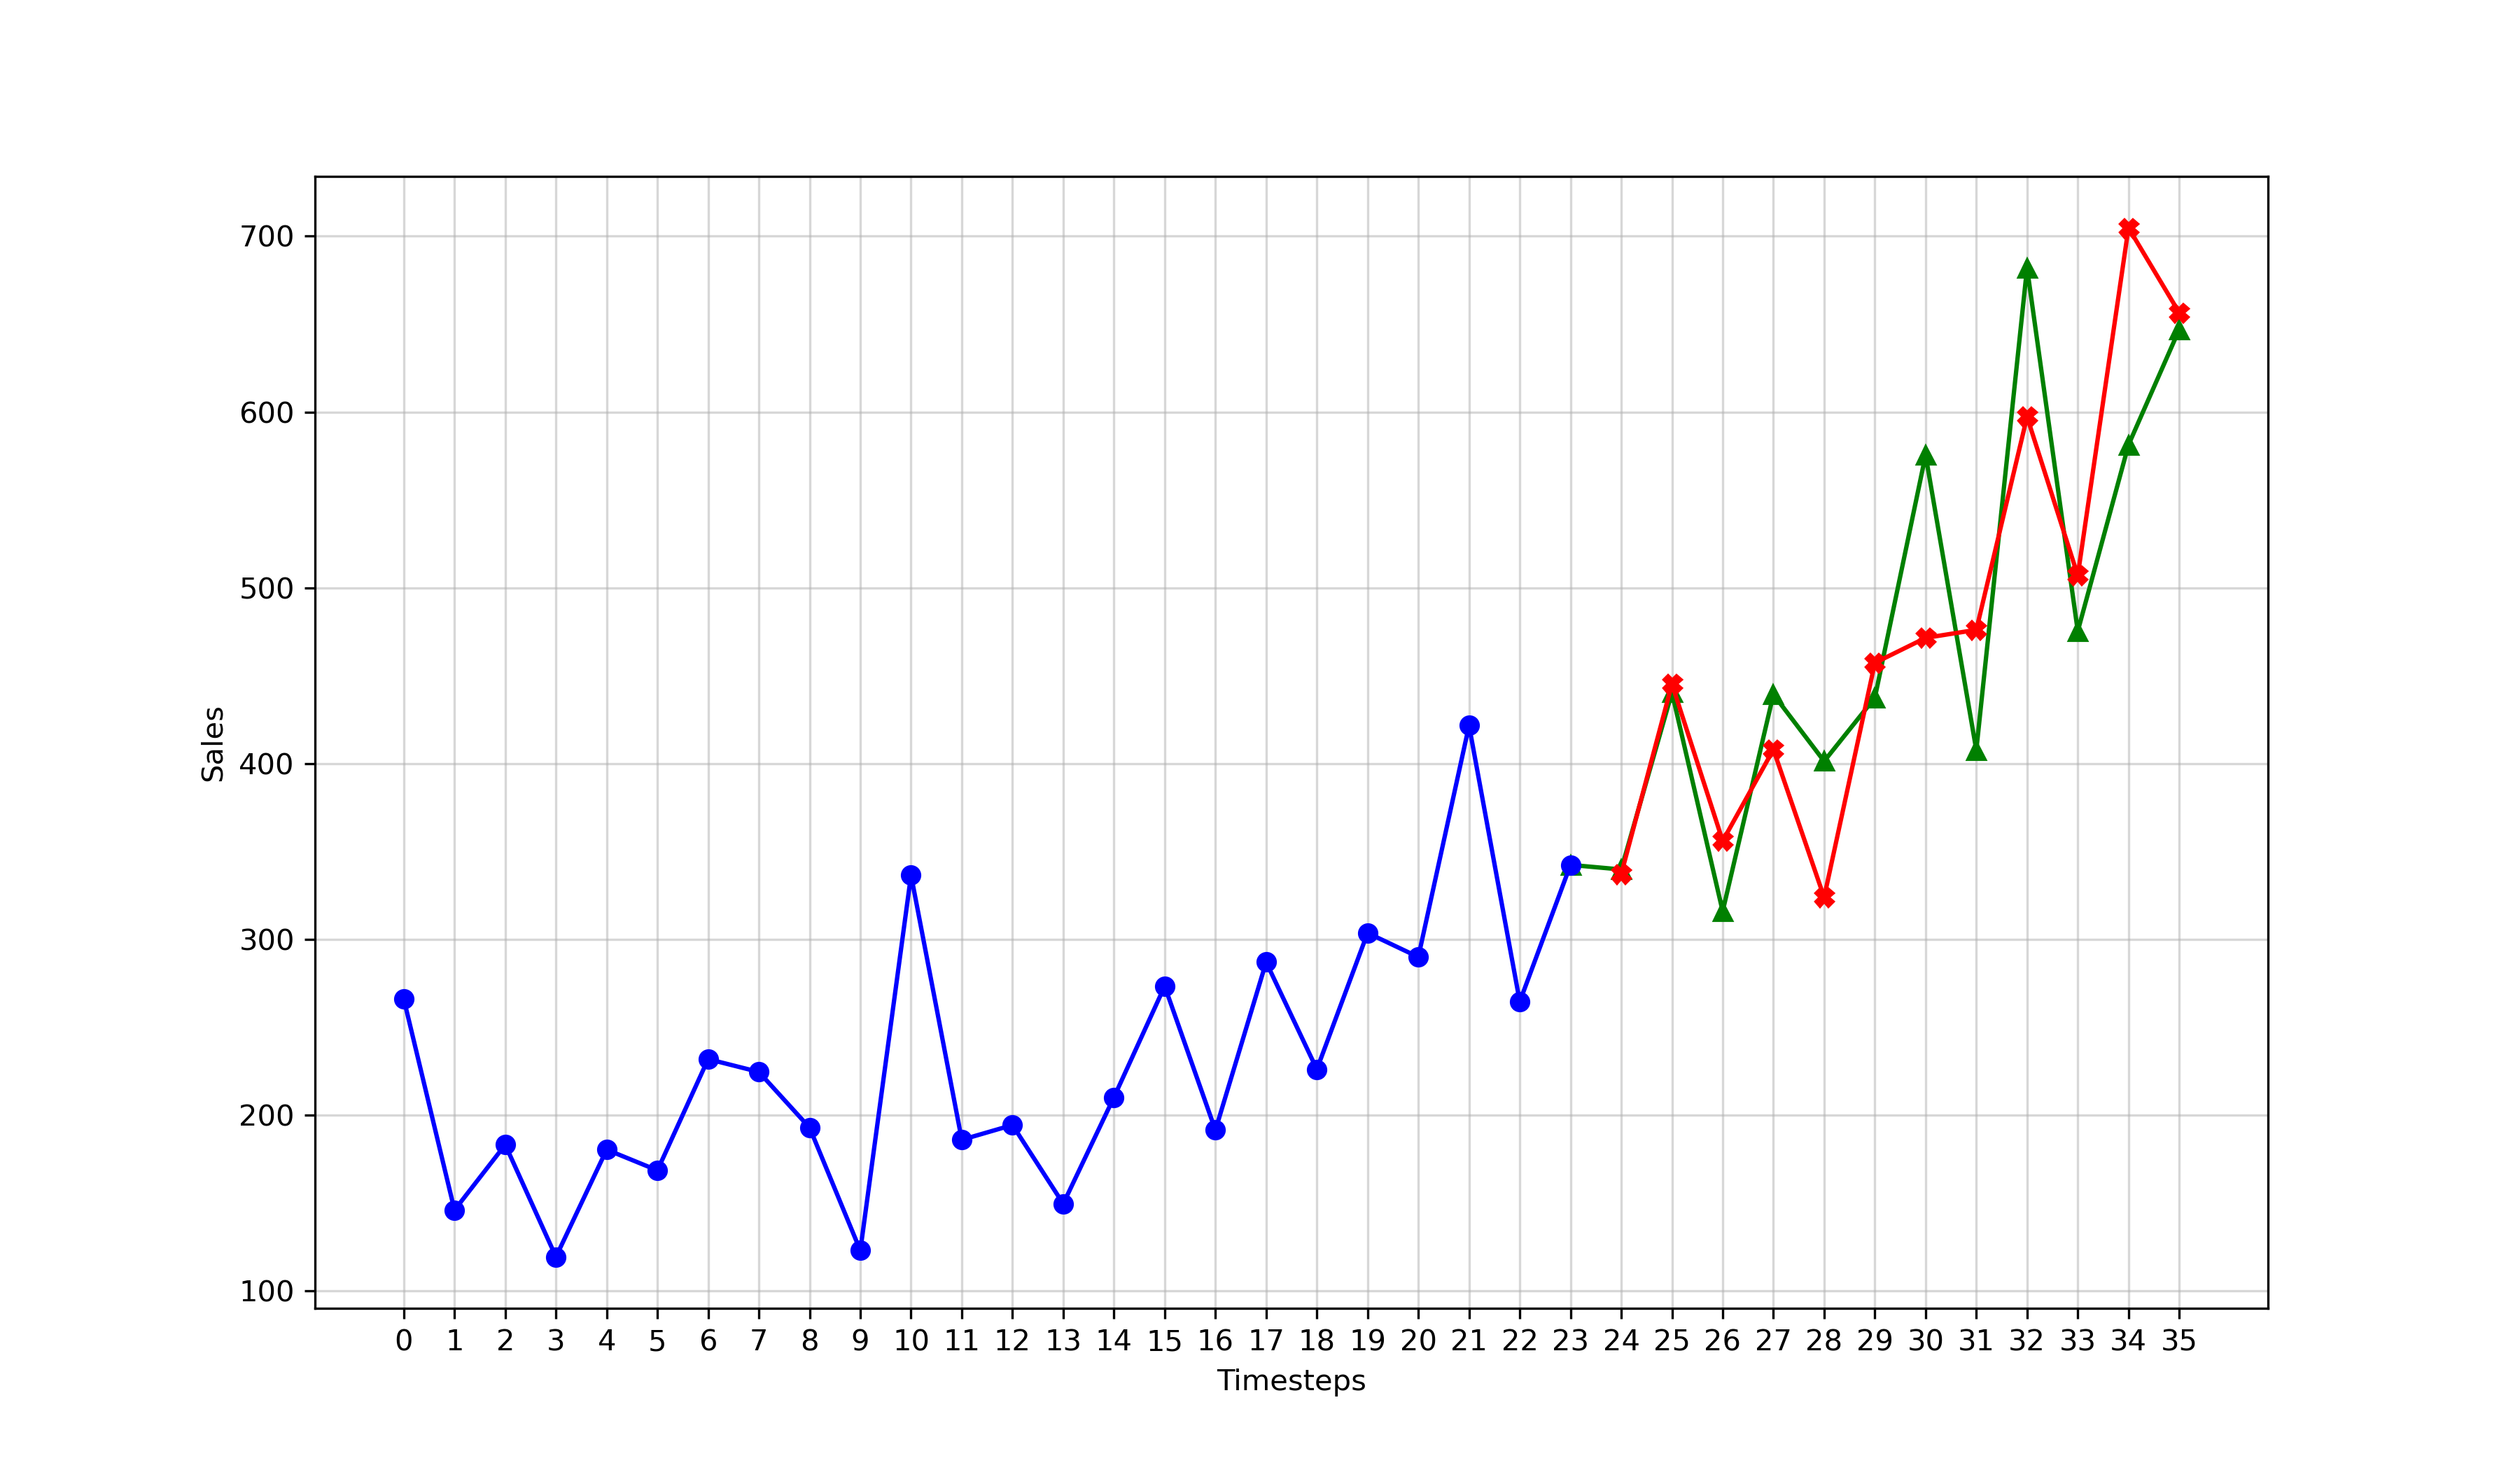
\includegraphics[width=\linewidth]{../private_assets/predictions_plot_example.png}
\caption{Gráfico de previsões de vendas de um champô}
\end{figure}\par

Como se pode observar na imagem, é necessário manter os dados de treino guardados, para
conseguir fazer previsões. Estes dados devem estar ordenados temporalmente. Visto que, 


\subsection{Univariada vs Multivariada}
O termo \say{série temporal univariada} refere-se a uma série temporal que consiste em
observações únicas (escalares) registadas sequencialmente em incrementos de tempo iguais.
Por exemplo, as concentrações mensais de \acrshort{co2} ou as medições das velocidades do
vento.\par Embora um \textit{\gls{dataset}} de uma série temporal univariada seja geralmente
fornecido como uma única coluna de dados, o tempo é, de facto, uma variável implícita na
série temporal\cite{univariate_multivariate}. Se os dados tiverem espaçamento igual, a variável de tempo, ou índice, não
precisa de ser fornecida explicitamente. Esta variável às vezes pode ser usada explicitamente
para traçar a série. No entanto, não é usada no próprio modelo. A tabela 2.1 demonstra um
excerto de uma série temporal univariada para servir de exemplo.\par

\begin{table}[h!]
\centering
\setlength{\extrarowheight}{5pt}
\setlength{\tabcolsep}{10pt}
\begin{tabular}{|c|c|}
\hline
\textbf{"date"} & \textbf{"census"} \\[5pt]
\hline
01/01/2016 & 4092 \\[5pt]
\thinhline
02/01/2016 & 3807 \\[5pt]
\thinhline
03/01/2016 & 3208 \\[5pt]
\thinhline
04/01/2016 & 1057 \\[5pt]
\thinhline
05/01/2016 & 3302 \\[5pt]
\thinhline
06/01/2016 & 3761 \\[5pt]
\thinhline
07/01/2016 & 2964 \\[5pt]
\hline
\end{tabular}
\caption{Excerto de série temporal univariada}
\end{table}
\vspace{15pt}

Por outro lado, uma série temporal multivariada abrange várias variáveis que são registadas
simultaneamente ao longo do tempo. Estas variáveis podem ou não contribuir para a previsão
do modelo. Na figura 2.2 pode ser visualizado um excerto de uma série temporal multivariada.
\par

\vspace{15pt}
\begin{table}[h!]
\centering
\setlength{\extrarowheight}{5pt}
\setlength{\tabcolsep}{10pt}
\begin{tabular}{|c|c|c|c|c|c|}
\hline
\textbf{"date"} & \textbf{"wifi status"} & \textbf{"temp"} & \textbf{"precipitation"} & \textbf{"census"} \\[5pt]
\hline
01/01/2016 & up & -6 & 0 & 4092 \\[5pt]
\thinhline
02/01/2016 & up & 2 & 0 & 3807 \\[5pt]
\thinhline
03/01/2016 & up & 2 & 0 & 3208 \\[5pt]
\thinhline
04/01/2016 & up & -4 & 0 & 1057 \\[5pt]
\thinhline
05/01/2016 & up & 2 & 0 & 3302 \\[5pt]
\thinhline
06/01/2016 & up & 2 & 0 & 3761 \\[5pt]
\thinhline
07/01/2016 & up & 4 & 0 & 2964 \\[5pt]
\hline
\end{tabular}
\caption{Excerto de série temporal multivariada}
\end{table}

\newpage
\section{Modelo ARIMA}
O modelo de Média Móvel Integrada Autoregressiva\cite{arima_forecast_python} - \textit{\acrfull{arima}} - foi o modelo
utilizado para realizar este trabalho, sendo que, todo o projeto foi abordado em torno
deste modelo e variações do mesmo\cite{arima_wiki}. \textit{\acrshort{arima}} significa:
\begin{itemize}
    \item AR: "\textit{Autoregression}" (Autoregressão) - Um modelo que usa a relação entre
    uma observação e um número de observações atrasadas;
    \item I: "\textit{Integrated}" (Integrado) - O uso de diferenciação de observações (por
    exemplo, retirar uma observação de uma observação, no passo anterior) de forma a manter
    a série temporal estacionária;
    \item MA: "\textit{Moving Average}" (Média Móvel) - Um modelo que usa a dependência
    entre uma observação e o erro residual de um modelo de média móvel aplicado a
    observações atrasadas.
\end{itemize}\par
O propósito de cada uma das características é fazer com que o modelo se ajuste aos dados da
melhor forma possível.\cite{econometric_analysis} Cada um destes componentes está especificado
no modelo como um parâmetro. A notação utilizada é $ARIMA(p, d, q)$:
\begin{itemize}
    \item p: Ordem de atraso - número de observações atrasadas incluídas no modelo;
    \item d: Grau de diferenciação - número de vezes que observações brutas são
    diferenciadas;
    \item q: Ordem da média móvel - tamanho da janela de media móvel.
\end{itemize}\par
Dado um conjungo de dados de uma série temporal $X_t$ onde $t$ é um índice inteiro e $X_t$ são
números reais, um modelo $ARMA(p', q)$ é dado por:\\[10pt]
\indent\begin{math}
    X_t - a_1 X_{t-1} - ... - a_{p'} X_{t-p'} = \varepsilon_t + \theta_1 \varepsilon_{t-1} + ... + \theta_q \varepsilon_{t-q'}
\end{math}\\[10pt]
\indent ou equivalentemente por:\\[10pt]
\indent\begin{math}
    (1 - \sum_{i=1}^{p'} \alpha_i L^i) X_t = (1 + \sum_{i=1}^q \theta_i L^i) \varepsilon_t
\end{math}\par


\section{Modelo ARIMAX}
O modelo de Média Móvel Integrada Autoregressiva com Variáveis Exógenas -
\textit{\acrfull{arimax}} - é bastante semelhante ao modelo \textit{\acrshort{arima}}.
Existem algumas diferenças, embora não seja tão aparente\cite{arimax_forecast}.\par
Os componentes deste modelo são os mesmos que os do modelo \textit{\acrshort{arima}} com o
acréscimo das \gls{variaveis exogenas}. Estas são variáveis cujos valores são determinados
fora do modelo e são impostas ao modelo (neste caso serão utilizadas para ajudar a fazer
as previsões).

\section{Modelo SARIMA}
O modelo de Média Móvel Integrada Autoregressiva Sazonal - \textit{\acrfull{sarima}} - é
bastante semelhante ao modelo \textit{\acrshort{arima}}. Existem mais diferenças que no
modelo \textit{\acrshort{arimax}}.\par
Os componentes deste modelo são os mesmos que os do modelo \textit{\acrshort{arima}} com o
acréscimo de um conjunto extra de parâmetros característico deste tipo de modelos\cite{sarima_site}. São elas:
\begin{itemize}
    \item P: Ordem de atraso sazonal;
    \item D: Grau de diferenciação sazonal;
    \item Q: Ordem da média móvel sazonal;
    \item S: Temporada - número de iterações por cada período sazonal (temporada).
\end{itemize}\par
Desta forma, o modelo será abordado com esta fórmula: $SARIMA(p, d, q)(P, D, Q, S)$. Este
modelo é representado pela seguinte equação matemática\cite{sarima_eq}:\\[10pt]
\indent\begin{math}
    (1-\phi_1B)(1-\Phi_1B^4)(1-B)(1-B^4)y_t = (1+\theta_1B)(1+\Theta_1B^4)e_t
\end{math}\\[10pt]


\section{Modelo SARIMAX}
O modelo de Média Móvel Integrada Autoregressiva Sazonal com Variáveis Exógenas -
\textit{\acrfull{sarimax}} - é uma junção dos modelos \textit{\acrshort{sarima}} e
\textit{\acrshort{arimax}}, visto que contém os parâmetros característicos dos
modelos \textit{\acrshort{sarima}} e ainda contém \gls{variaveis exogenas}\cite{sarimax}.


\newpage
\section{Grid Search}
\textit{\Gls{grid search}} (ou pesquisa em grelha) é o processo de coleção de dados para
configurar os parâmetros ideais para um determinado modelo\cite{grid_search}. Dependendo do tipo de modelo
utilizado, alguns parâmetros são necessários. Esta pesquisa não se aplica apenas a um
tipo de modelo, ela pode ser aplicada ao modelo de aprendizagem para calcular os melhores
parâmetros a serem usados para qualquer modelo. Um exemplo desta pesquisa pode ser
visualizado na figura 2.3, na qual está representado um mapa de calor resultante de uma
\textit{\gls{grid search}} de parâmetros de um modelo.\par

\begin{figure}[h!]
\centering
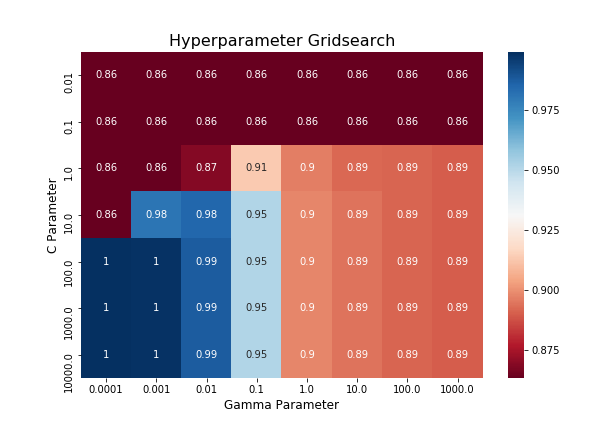
\includegraphics[width=0.9\linewidth]{../private_assets/grid_search_example.png}
\caption{Mapa de calor representativo de uma \textit{\gls{grid search}} de parâmetros de
um modelo}
\end{figure}\par

Um ponto importante a sublinhar é que esta pesquisa pode ser extremamente cara em
termos computacionais e pode levar muito tempo até obter resultados. O \textit{grid search}
construirá um modelo em cada combinação de parâmetros possível. Ele itera por meio de cada
combinação de parâmetros e armazena um modelo para cada combinação.


\newpage
\section{Tecnologias Utilizadas}

\subsection{Linguagens de Programação}
Para a realização deste projeto foi utilizada a linguagem \textit{\gls{python}}, visto
que é uma das ou a melhor linguagem para realizar projetos de investigação de algoritmos
de aprendizagem, pela enormíssima vasta gama de bibliotecas fortíssimas, bastante úteis
e adaptadas para o progresso do trabalho.\par
O \textit{\gls{python}} é também uma linguagem bastante utilizada pela comunidade de
desenvolvedores de software, ou seja, encontrar soluções para problemas que ocorram não
será muito árduo.\par

\subsection{Ambiente de Desenvolvimento}
Com a finalidade de obter um bom, compacto e replicável ambiente de desenvolvimento, foi
criado um ambiente de desenvolvimento virtual com \textit{\gls{python}} e instaladas as
dependências presentes no ficheiro \textit{\say{requirements.txt}} presente na pasta
principal do projeto.\par
Feito isto, foi utilizado o \textit{\acrshort{ide}} \textit{PyCharm} e o editor de
código fonte \textit{Visual Studio Code}. As tecnologias utilizadas no decorrer de todo
o trabalho estão representadas na figura 3.3.\par

\vspace{10pt}
\begin{figure}[h!]
\centering

\includegraphics[width=0.5\linewidth]{../public_assets/Stack.png}
\caption{\textit{Stack} tecnológica do projeto}
\end{figure}

\newpage